\section{Quine-McCluskey}

\subsection{Treść zadania}

\begin{figure}[h!]
    \centering
    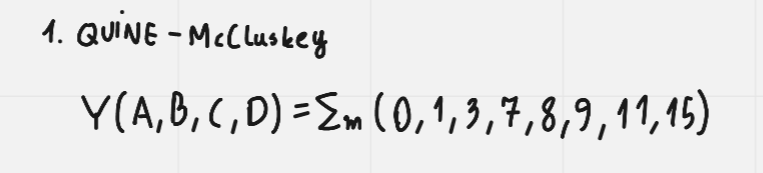
\includegraphics[width=.8\textwidth]{images/qmc/qmc_ex.png}
    \caption{treść zadania}
    \label{fig:my_label}
\end{figure}

\vspace{0.5cm}

\raggedright

Funkcja Y dla zmiennych ABCD przyjmuje wartości 1 dla słów 0,1,3,7,8,9,11,15. A jest najstarszym bitem a D najmłodszym.

\subsection{Rozwiązanie}

\subsubsection{Małe kotki}

Każdemu słowu przypisujemy grupę która oznacza ilość wystąpień jedynek w słowie: \textbf{grupa pierwsza (g 1)} to słowo mające zero jedynek, a \textbf{grupa czwarta (g 4)} trzy jedynki.

\begin{figure}[h!]
    \centering
    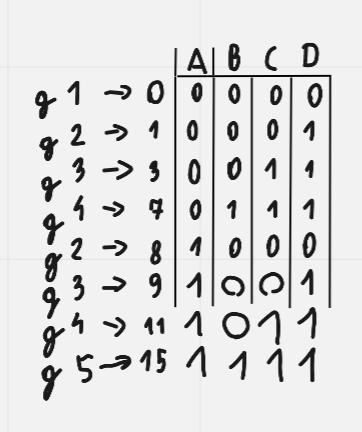
\includegraphics[width=0.45\textwidth]{images/qmc/qmc_0.png}
    \caption{małe kotki}
    \label{fig:my_label}
\end{figure}

\newpage

\subsubsection{Pluszowe misie}

Przepisujemy tabelkę tak jak przedstawione to na rysunku - poszczególne grupy są oddzielone od siebie żeby ułatwić następne etapy.

\begin{figure}[h!]
    \centering
    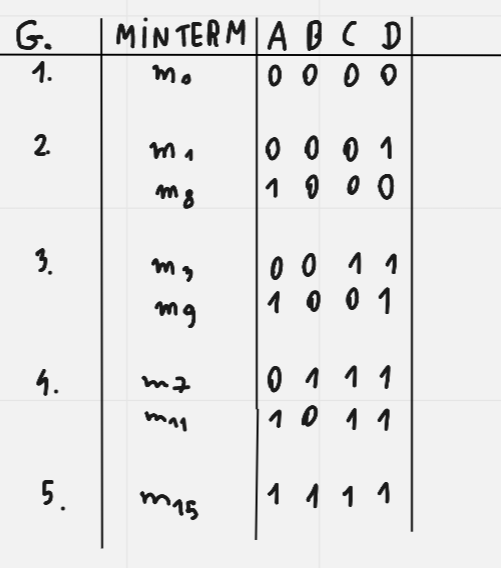
\includegraphics[width=0.4\textwidth]{images/qmc/qmc_1.png}
    \caption{pluszowe misie}
    \label{fig:my_label}
\end{figure}

\subsubsection{Składnik X}

Słowa które znajdują się w różnych grupach i różnią się od siebie jednym bitem łączymy w pary przepisując je do kolejnej tabeli, wyrażenia przepisujemy bez zmian a na bicie który się różnił wpisujemy symbol podłogi

\begin{figure}[h!]
    \centering
    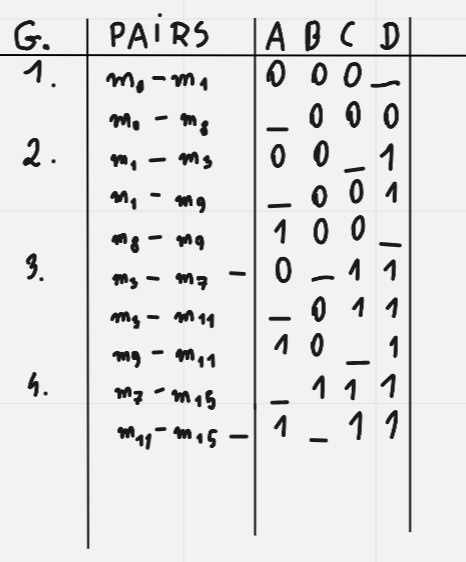
\includegraphics[width=0.4\textwidth]{images/qmc/qmc_2.png}
    \caption{składnik X}
    \label{fig:my_label}
\end{figure}

\subsubsection{Szalony naukowiec}

Nasze pary łączymy następnie w czwórki, stosując dokładnie tą samą metodę, mechanizm ten powtarzamy, póki możliwe jest uszczuplenie tabelki.\\ po maksymalnej optymalizacji naszej tabeli, łącząc klamrami wyrażenia z tych samych grup wpisujemy wyrażenia boolowskie analogicznie do siatek Karnaugha.

\begin{figure}[h!]
    \centering
    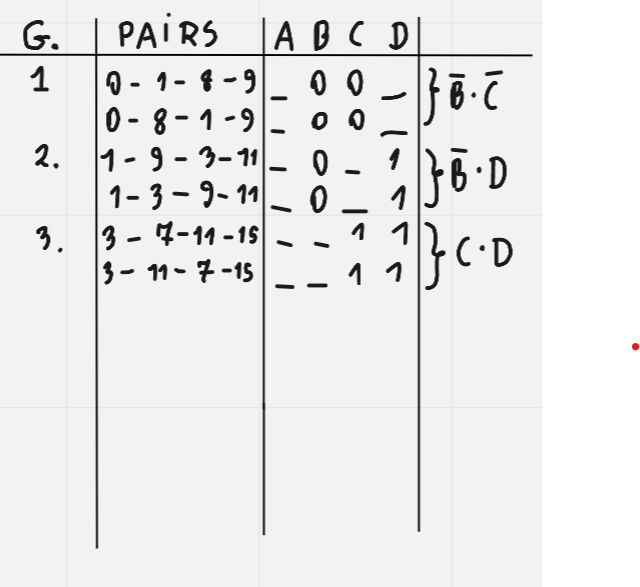
\includegraphics[width=0.45\textwidth]{images/qmc/qmc_3.png}
    \caption{szalony naukowiec}
    \label{fig:my_label}
\end{figure}

\subsubsection{Magiczna tabelka}

Tworzymy tabelkę tak jak poniżej. W kolumnach szukamy pojedynczych X. Wiersze w których nie występują zaznaczone krzyżyki odrzucamy i zapisujemy wyrażenie (analogicznie do siatek karnaugha)

\begin{figure}[h!]
    \centering
    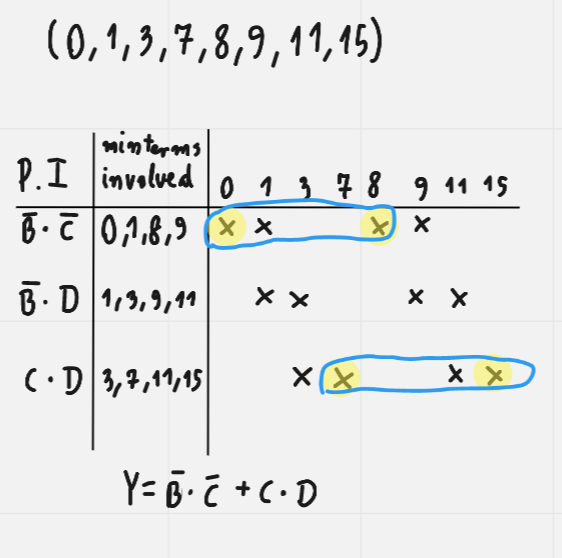
\includegraphics[width=0.50\textwidth]{images/qmc/qmc_4.png}
    \caption{magiczna tabelka}
    \label{fig:my_label}
\end{figure}

\newpage

\subsection{Rozwiązanie siatką karnaugha}

\begin{figure}[h!]
    \centering
    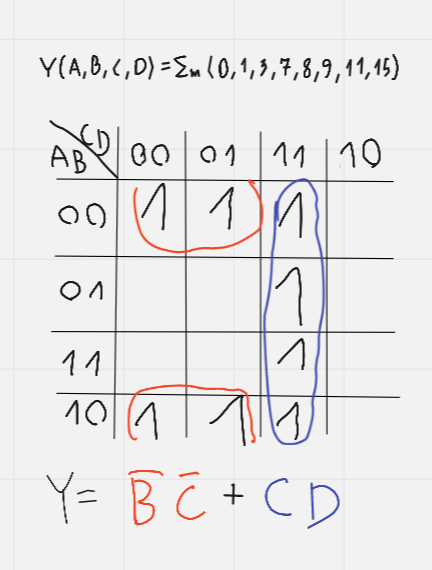
\includegraphics[width=0.4\textwidth]{images/qmc/qmc_k.png}
    \caption{rozwiązanie siatką karnaugha}
    \label{fig:my_label}
\end{figure}

\subsection{Klik}

\url{http://quinemccluskey.com/}